\begin{frame}
\frametitle{Математическая модель интерферометра Маха-Цендера без линз}
\begin{columns}
\column{0.6\linewidth}
  \centering
  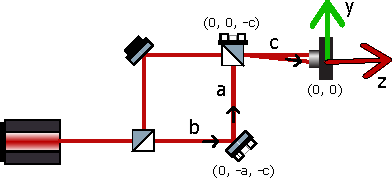
\includegraphics[width=1\linewidth]{images/MZI_matmodel.pdf}
  \begin{itemize}
    \item управление положением луча на камере $(x_0, y_0)$
    \item управление направлением $\vec{k}$
  \end{itemize}

\column{0.5\linewidth}
\begin{table} [htbp]
    \centering
    \begin{threeparttable}
        \begin{tabular}{| p{2.5cm} || p{2cm} |}
            \hline
            \hline
            параметр & значение \\
            \hline
            Mirror 2 $\to$ BS 2 & 200 mm\\
            BS 1 $\to$ Mirror 2 & 300 mm\\
            BS 2 $\to$ Camera & 100 mm\\
            radius & 0.95\\
            $\alpha_{{\mathrm{max}}(x,1)}$ & $5.2 \cdot 10^{-3}$ rad\\
            $\alpha_{{\mathrm{max}}(y,1)}$ & $3.7 \cdot 10^{-3}$ rad\\
            $\alpha_{{\mathrm{max}}(x,2)}$ & $2.6 \cdot 10^{-3}$ rad\\
            $\alpha_{{\mathrm{max}}(y,2)}$ & $1.8 \cdot 10^{-3}$ rad\\
            \hline
            \hline
        \end{tabular}
    \end{threeparttable}
\end{table}

\end{columns} 
\end{frame}


\begin{frame}
\frametitle{Примеры интерференционных картин без линз полученные в симуляции}
\begin{columns}
\column{0.7\linewidth}
  \centering
   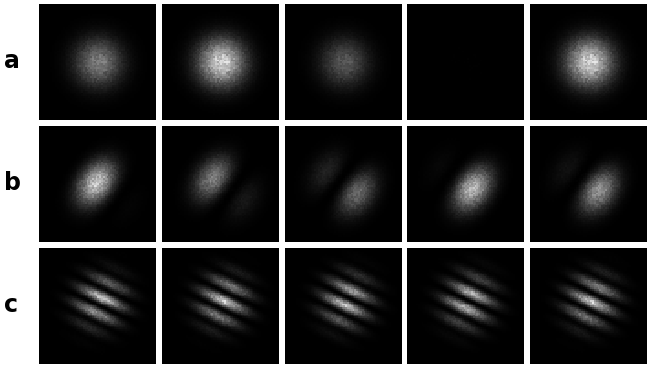
\includegraphics[scale=0.4]{images/visib_expl.png}

\column{0.5\linewidth}
\begin{description}
    \item V = 1
    \vspace{30pt}
    \item V = 0.3
    \vspace{30pt}
    \item V = 0.0026
\end{description}

\end{columns} 
\end{frame}


\begin{frame}
\frametitle{Математическая модель интерферометра Маха-Цендера с линзами}
\begin{columns}
\column{0.6\linewidth}
  \centering
   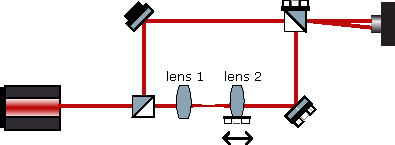
\includegraphics[width=1\linewidth]{images/MZI_expl_lenses.pdf}
  \begin{itemize}
    \item управление положением луча на камере $(x_0, y_0)$
    \item управление направлением $\vec{k}$
    \item \textcolor{red}{управление волновым фронтом}
  \end{itemize}

\column{0.5\linewidth}
\begin{table} [htbp]
    \centering
    \begin{threeparttable}
        \begin{tabular}{| p{2.5cm} || p{2cm} |}
            \hline
            \hline
            параметр & значение \\
            \hline
            BS 1 $\to$ Lens 1 & 50 mm\\
            $f_{\mathrm{lens 1}}$ = $f_{\mathrm{lens 2}}$ & 50 mm\\
            radius & 0.71 mm\\
            $\Delta_{\mathrm{max}}$ & 4.2 mm\\
            \hline
            \hline
        \end{tabular}
    \end{threeparttable}
\end{table}

\end{columns} 
\end{frame}

\begin{frame}
    \frametitle{Примеры интерференционных картин полученные на интерферометре Маха-Цендера с линзами}
    \centering
    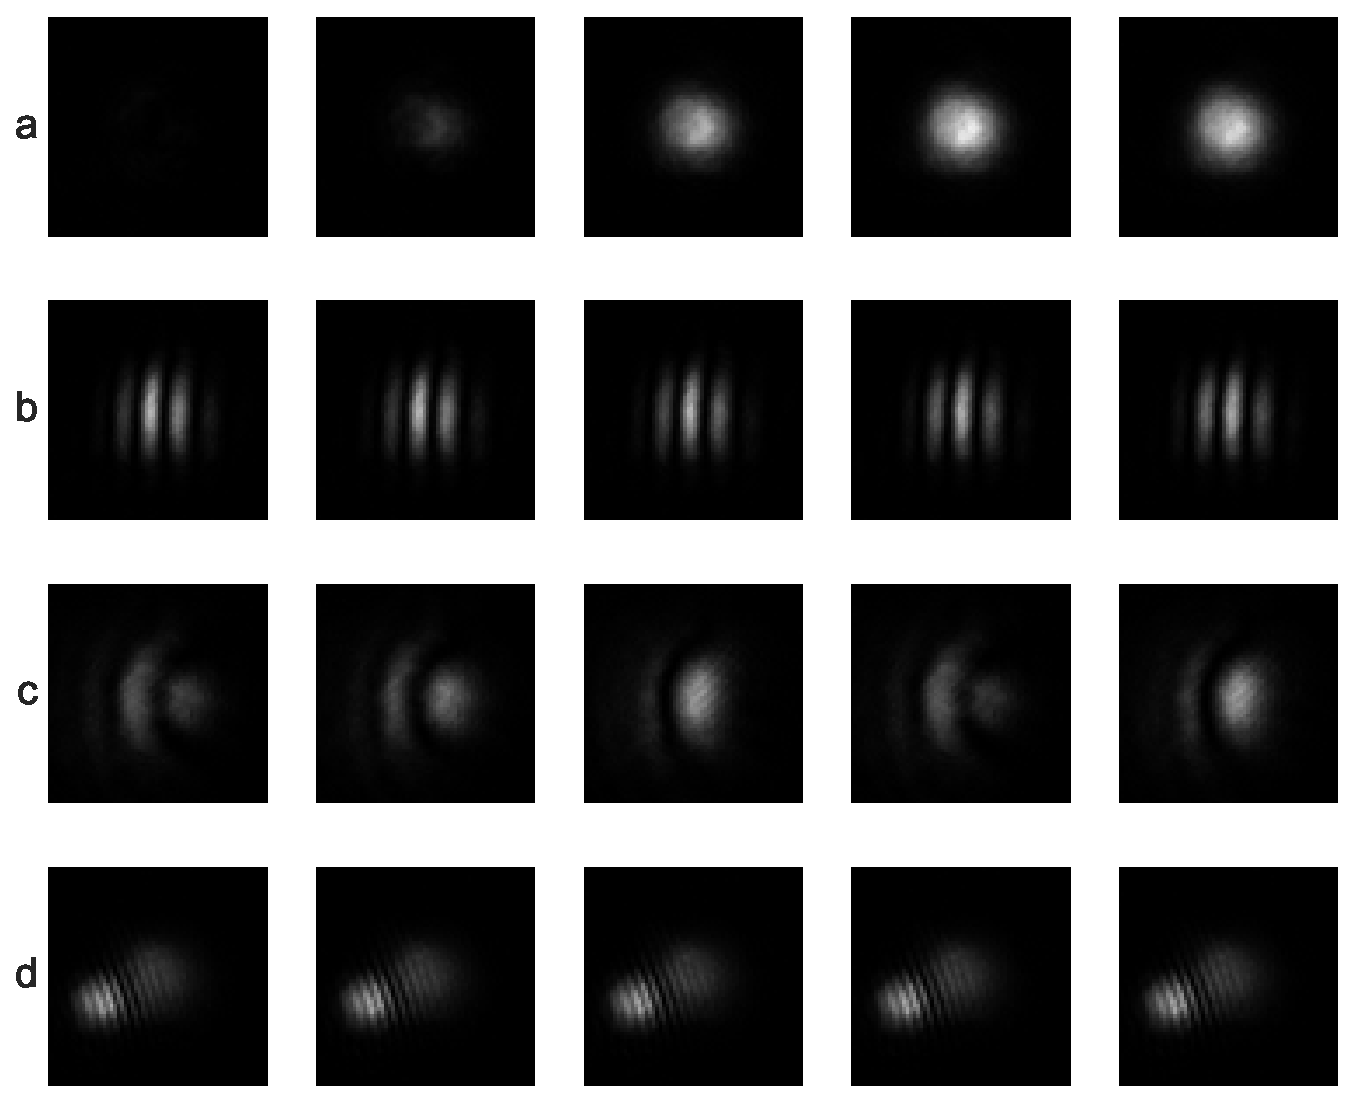
\includegraphics[width=0.8\linewidth]{images/Env_patterns.pdf}
\end{frame}

\begin{frame}
\frametitle{Видность интерференционной картины в интерферометре
Маха-Цендера без линз}

\begin{columns}
\column{0.4\linewidth}
\centering
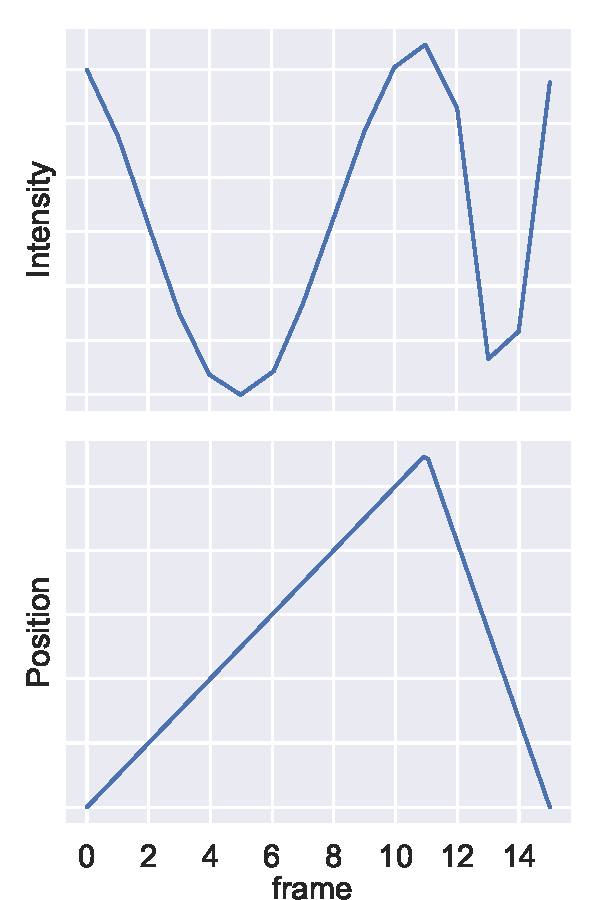
\includegraphics[width=1\linewidth]{piezo.pdf}

\column{0.5\linewidth}
\begin{align*}
& I(x,y,t)=|E_1(x,y,0)+E_2(x,y,0)e^{i\phi_{\mathrm{piezo}}(t)}|^2 \\
& I_{\mathrm{tot}}(t) = \iint_{-\infty}^{+\infty} I(x, y, t) {\mathrm{d}}x{\mathrm{d}}y \\
& V = \frac{            
        \max_{t}(I_{\mathrm{tot}}) - \min_t(I_{\mathrm{tot}})}
        {\max_{t}(I_{\mathrm{tot}}) + \min_t(I_{\mathrm{tot}})} \\
& V = \exp\left(- \frac{x_0^2 + y_0^2}{2 r^2}\right)  \exp\left[- \frac{(k_x^2 + k_y^2) r^2}{8}\right] \\
\end{align*}

\end{columns}
\end{frame}

\begin{frame}
\frametitle{Видность интерференционной картины в интерферометре Маха-Цендера с линзами}
\begin{columns}
\column{0.3\linewidth}
\begin{align*}
& \dfrac{1}{q} = \dfrac{1}{\rho} - \dfrac{i \lambda}{\pi r^2} \\
& q^{\prime}=\dfrac{A q+B}{C q+D}\\
\end{align*}
\column{0.7\linewidth}
\begin{align*}
& \begin{bmatrix} A & B \\ C & D \end{bmatrix}=\begin{bmatrix} 1 & d \\ 0 & 1 \end{bmatrix} \hspace{25pt}\text{вакуум длины $d$}\\
& \begin{bmatrix} A & B \\ C & D \end{bmatrix}=\begin{bmatrix} 1 & 0 \\ -1/f & 1 \end{bmatrix} \hspace{5pt}\text{линза с фокусным расстоянием $f$} \\
& M = M_3^{ABCD} \times M_2^{ABCD} \times M_1^{ABCD}
\end{align*}
\end{columns}

\begin{equation*}
\begin{split}
    V =\frac{4}{\left(n^{2}+1\right) r_{\mathrm{u}}^{2}} \frac{1}{c} \exp \left(-\left(x_{0}^{2}+y_{0}^{2}\right)\left(\frac{1}{r_{\mathrm{u}}^{2} n^{2}}-\frac{n^{2}+1}{n^{6} r_{\mathrm{u}}^{6} c^{2}}\right)\right) \times \\ \times \exp \left(-\frac{n^{2}+1}{4 c^{2} n^{2} r_{\mathrm{u}}^{2}}\left(k_{x}^{2}+k_{y}^{2}\right)\right) \exp \left(\frac{\frac{\pi}{\lambda \rho^{\prime}}}{n^{2} r_{\mathrm{u}}^{2} c^{2}}\left(x_{0} k_{x}+y_{0} k_{y}\right)\right),
\end{split}
\end{equation*}
параметр $n=\dfrac{r_{\mathrm{l}}}{r_{\mathrm{u}}}$, $c^2 = (\dfrac{n^2 + 1}{n^2r^2_{\mathrm{u}}})^2$
\end{frame}

\begin{frame}{Анализ стратегии дискретного DQN агента}

\begin{minipage}{\textwidth}
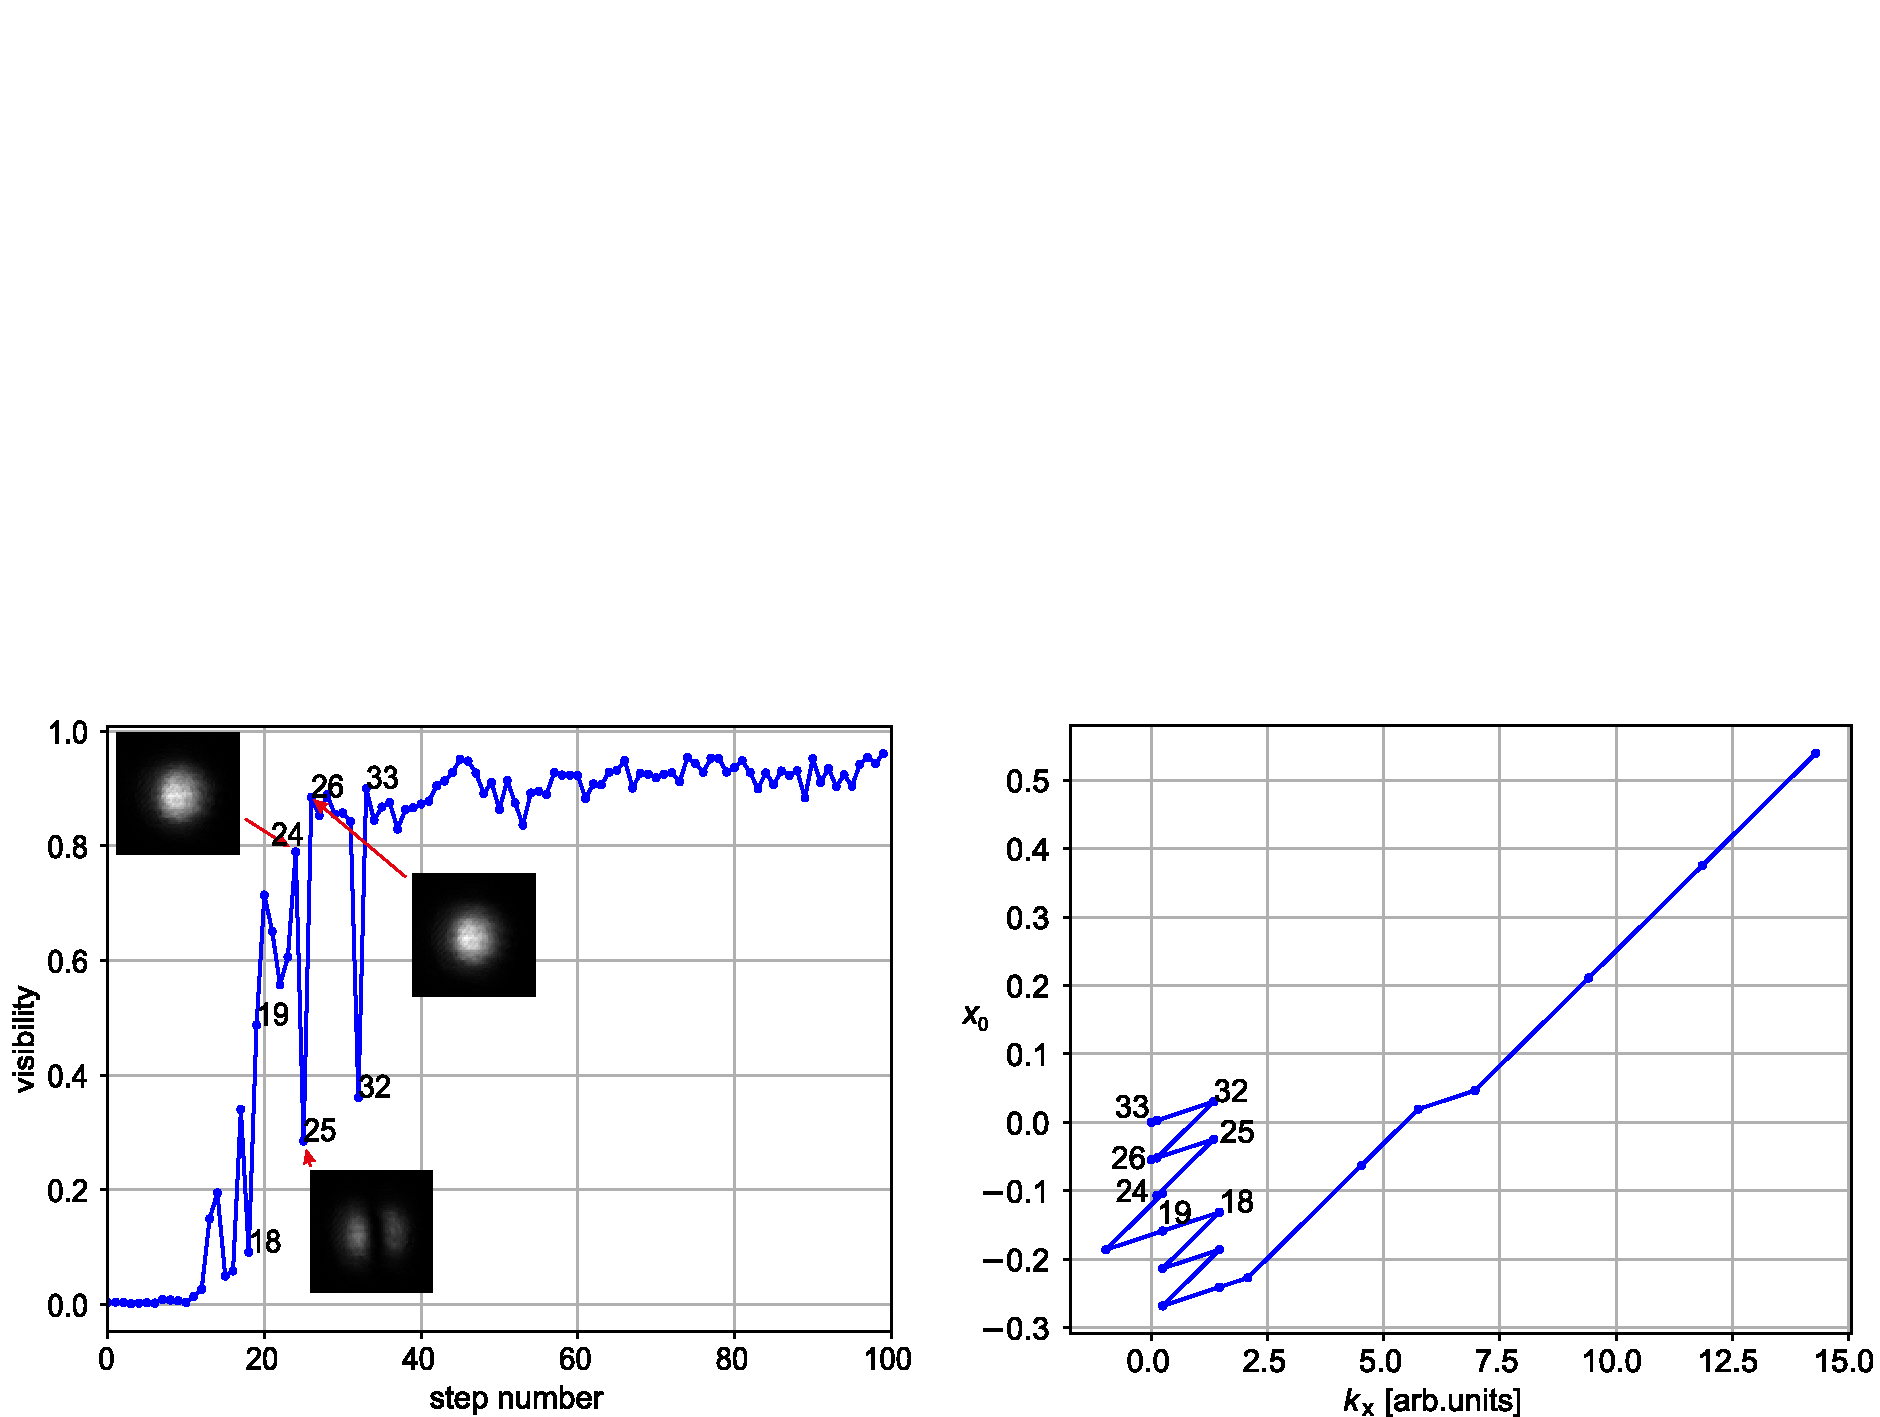
\includegraphics[width=1\linewidth]{DQN_analysis.pdf}
\end{minipage}
\begin{minipage}{\textwidth}
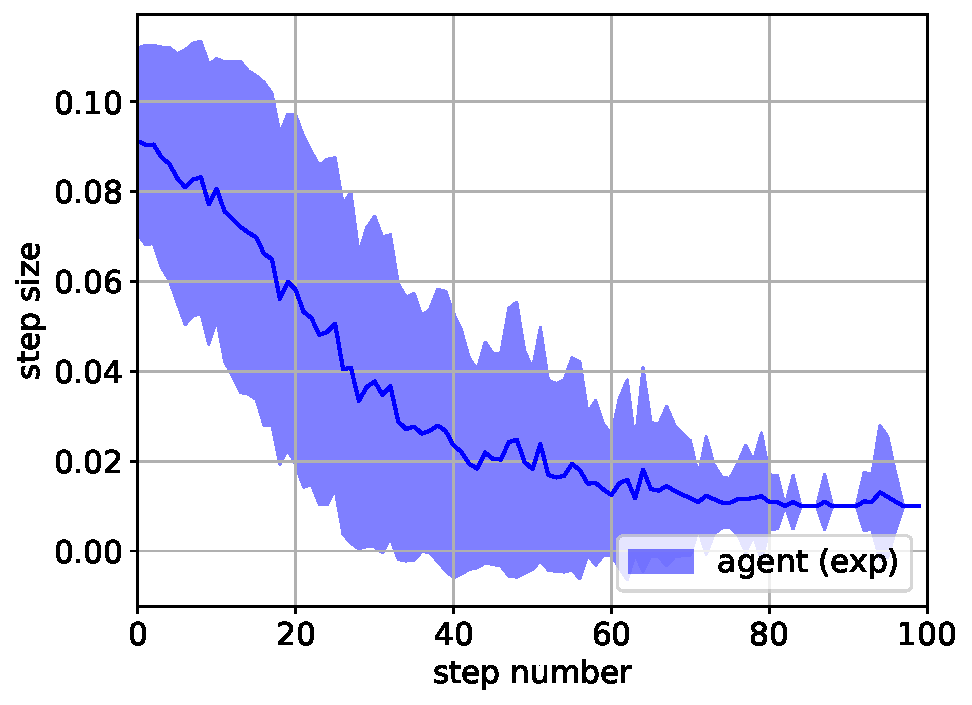
\includegraphics[width=0.5\linewidth]{images/agent_step_size.pdf}
\end{minipage}
\end{frame}

\begin{frame}{Анализ стратегии непрерывного TD3 агента}
\begin{columns}
\column{0.5\linewidth}
\centering
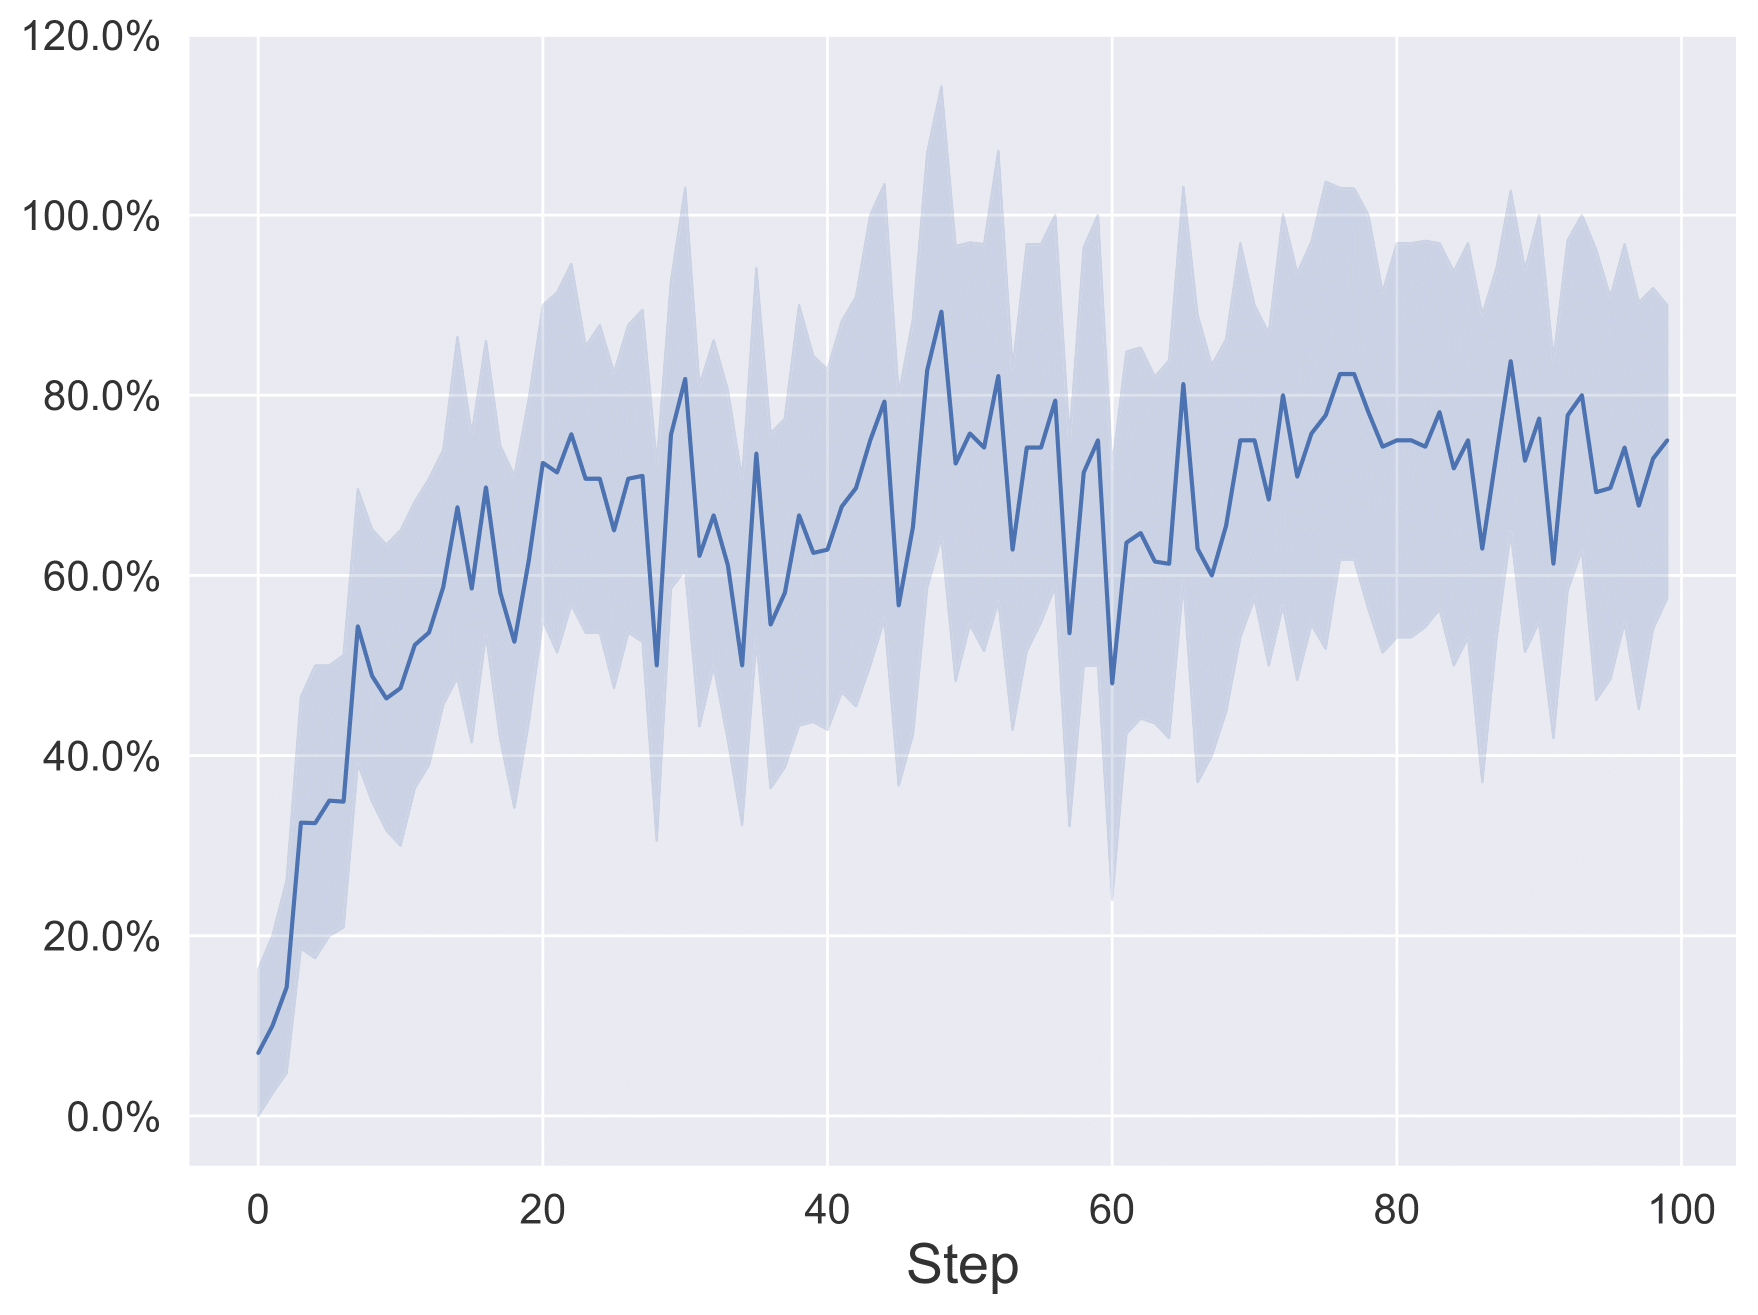
\includegraphics[width=1\linewidth]{Presentation/images/parallel_actions.png}
Процент "параллельных действий"
\column{0.5\linewidth}
\centering
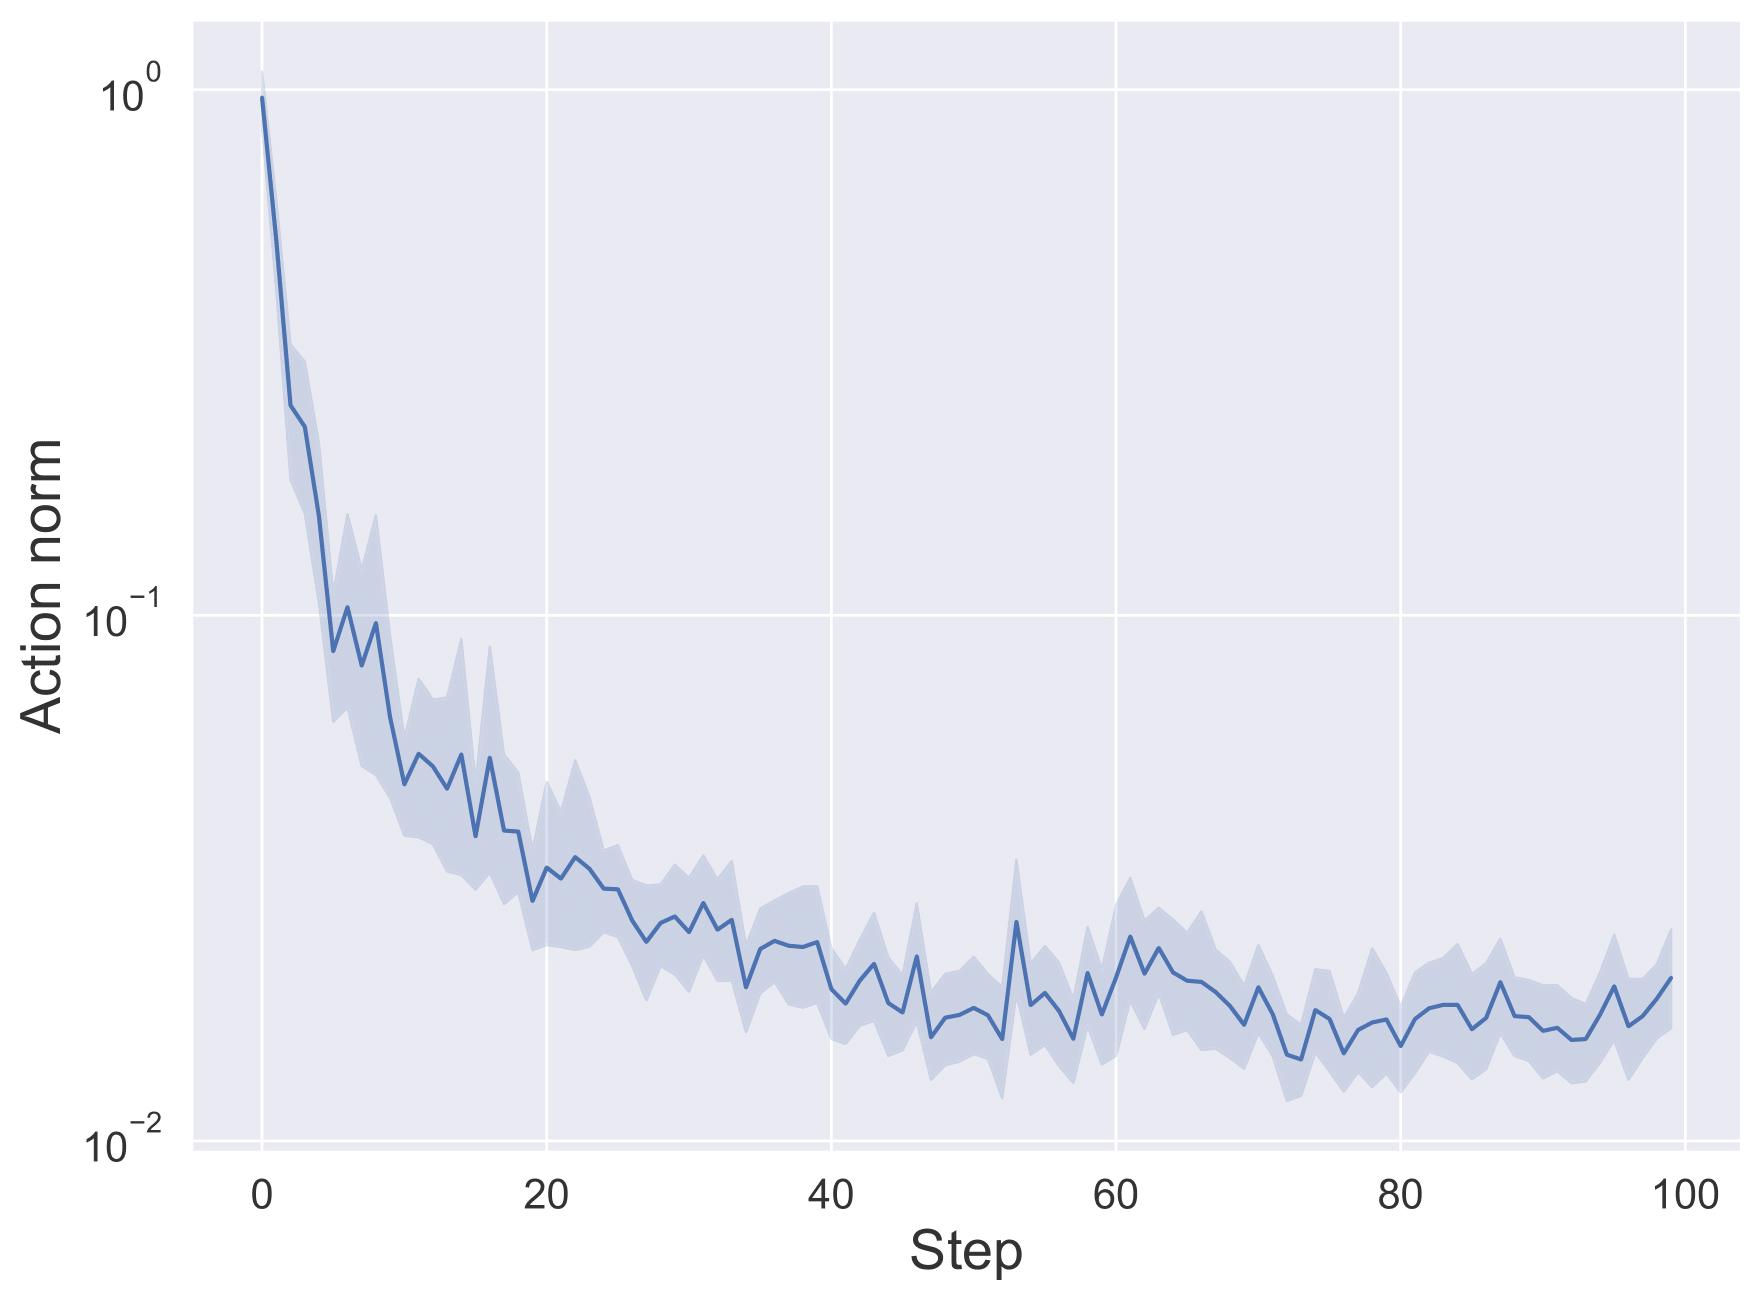
\includegraphics[width=1\linewidth]{Presentation/images/action_norm_decrease.png}
Средняя амплитуда действий
\end{columns}
\end{frame}

\begin{frame}{Управляющие элементы интерферометра}
\begin{columns}
\column{0.5\linewidth}
\centering
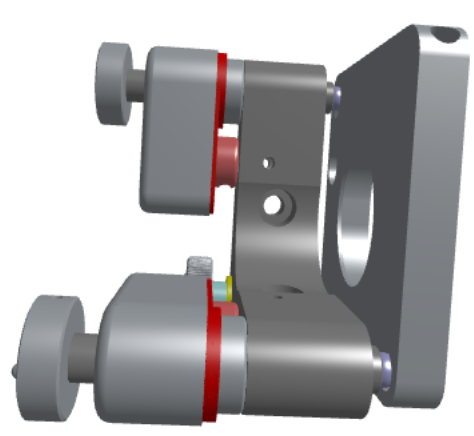
\includegraphics[width=0.7\linewidth]{images/mirror_mount.png}\\
3D модель крепления оптического зеркала.
\column{0.5\linewidth}
\centering
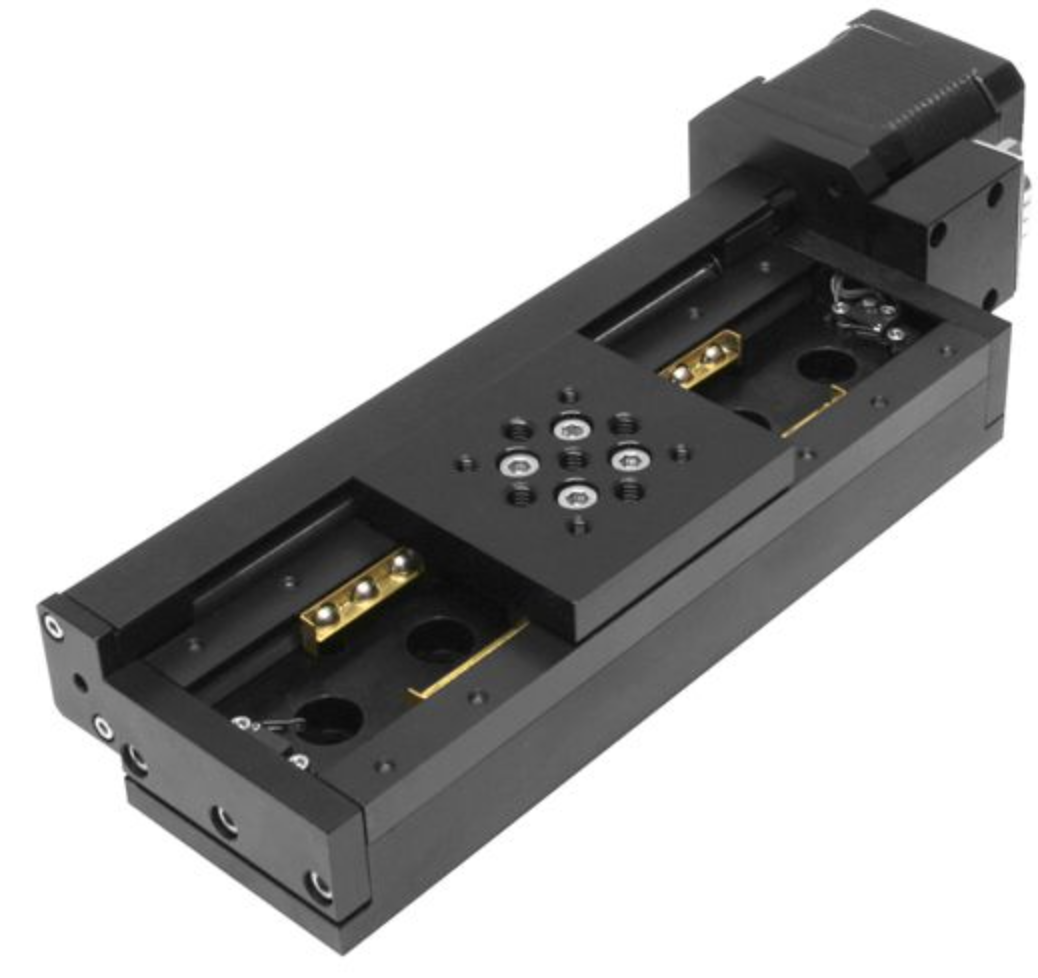
\includegraphics[width=0.7\linewidth]{images/lense_mount.png}
Подвижка, регулирующая положение линзы.
\end{columns}
\end{frame}

\begin{frame}{Репортаж 1 канала}
    
\end{frame}

\begin{frame}
    \frametitle{Научная новизна}
    \begin{itemize}
        \item Разработанный метод обучения с подкреплением, способный оперировать действиями различного масштаба и устойчивый к оптическим шумам, впервые был применен для настройки оптического интерферометра.
        \item Впервые создан программно-аппаратный комплекс настройки оптического интерферометра по изображениям с камеры, основанный на машинном обучении с подкреплением.
        \item Был разработан метод, позволяющий достичь сходимости к хорошему оптимутму для многозадачного агента. Разработанный метод был применен для управления движением шагающего робота с заданной линейной и угловой скоростью.
        \item Была предложена идея иерархического алгоритма, сочетающего в себе машинное обучения с подкреплением и запрограммированное поведение. 
        Разработанный алгоритм был применен для управления агентом в игре NetHack. 
    \end{itemize}
\end{frame}
\note{
    Проговаривается вслух научная новизна
}

\begin{frame}
    \frametitle{Научная и практическая значимость}
    \begin{itemize}
        \item Применение предложенного в работе автоматизированного подхода к настройке оптического интерферометра позволит существенно ускорить проведение физических экспериментов и снизит необходимость в ручном труде.
        \item Разработанные алгоритмы для управления виртуальными агентами затем могут быть применены в робототехнике, самоуправляемых автомобилях и виртуальных ассистентах.
    \end{itemize}
\end{frame}
\note{
    Проговариваются вслух научная и практическая значимость
}


%\begin{frame}
%    \frametitle{Ответы на замечания ведущей организации %НИИ~<<Рога~и~копыта>>}
%    \begin{itemize}
%        \item Замечание -- ответ
%        \item Замечание -- ответ
%        \item Замечание -- ответ
%        \item Замечание -- ответ
%        \item Замечание -- ответ
%    \end{itemize}
%\end{frame}

%\begin{frame}
%    \frametitle{Ответы на замечания оф. оппонента %Иванова\,И.\,И}
%    \begin{itemize}
%        \item Замечание -- ответ
%        \item Замечание -- ответ
%        \item Замечание -- ответ
%        \item Замечание -- ответ
%        \item Замечание -- ответ
%    \end{itemize}
%\end{frame}

%\begin{frame}
%    \frametitle{Ответы на замечания Петрова\,П.\,П}
%    \begin{itemize}
%        \item Замечание -- ответ
%        \item Замечание -- ответ
%        \item Замечание -- ответ
%        \item Замечание -- ответ
%        \item Замечание -- ответ
%    \end{itemize}
%\end{frame}
